% Math Notes by Rafid Ahsan
% Licensed under the GNU General Public License v3.0 or later
% See https://www.gnu.org/licenses/gpl-3.0.html for details

\chapter{Set Theory}

\section{Introduction}

In mathematics, we encounter a wide variety of objects. Set theory provides a fundamental framework for constructing these objects, while logic helps us distinguish and describe any equivalent relationships between them. In this section, we will acquaint ourselves with the essential concepts of set theory and the basics of logical reasoning.
\newline
\section{Sets}

\begin{definitionbox}{Set}
A \textbf{set} is a collection of objects, called \textbf{elements}. We denote a set by curly braces, \(\{\}\), and list the elements inside.

\begin{itemize}
    \item If an item \(a\) belongs to the set \(P\), we denote it by \(a \in P\). If an item \(b\) does not belong to the set \(P\), we denote it by \(b \notin P\).
    
    \item A set may be constructed using \textbf{set builder notation} as follows. Suppose \(P\) is our set. Then, we can write
    \[
    P = \{x \mid \text{some condition } C \text{ is true for } x\},
    \]
    where \(x\) is an element from a specified domain. This is read as "The set of all \(x\) such that some condition \(C\) is satisfied."

    \item We denote the \textbf{empty set} by \(\emptyset\) or \(\{\}\).
\end{itemize}
\end{definitionbox}


\begin{example}
\samepage
Some common examples of sets are:
\begin{itemize}
    \item The set of natural numbers: \(\mathbb{N} = \{1, 2, 3, \ldots\}\).
    \item The set of integers: \(\mathbb{Z} = \{\ldots, -2, -1, 0, 1, 2, \ldots\}\).
    \item The set of rational numbers: \(\mathbb{Q} = \left\{\frac{a}{b} \mid a, b \in \mathbb{Z}, b \neq 0\right\}\).
    \item The set of real numbers: \(\mathbb{R} = \{x \mid x \text{ is a real number}\}\).
\end{itemize}
\end{example}

\begin{example}
The set \(\mathcal{V}\) of all English vowels can be written as
\[
\mathcal{V} = \{a, e, i, o, u\}.
\]
\end{example}

\begin{example}
A \textbf{\textit{collection}} refers to a set whose \textit{elements are themselves sets}. Consider the following sets:

\[
E = \{2, 4, 6, 8, \dots\}, \quad O = \{1, 3, 5, 7, \dots\}, \quad P = \{2, 3, 5, 7, 11, \dots\}
\]

where:
\begin{itemize}
    \item \(E\) is the set of all \textbf{even natural numbers},
    \item \(O\) is the set of all \textbf{odd natural numbers}, and
    \item \(P\) is the set of all \textbf{prime numbers}.
\end{itemize}

We can now define a new set \(X\) as a \textit{collection of sets}:

\[
X = \{E, O, P\}
\]

Here, each element of \(X\) is itself a set. Thus, \(X\) is a \textit{collection of sets}. For example, the element \(E \in X\) represents the set of all even numbers.

Notice that:
\[
x \in X \implies x \text{ is a set}.
\]

Sets are not restricted to containing only numbers. As demonstrated in the previous examples, sets can comprise a wide variety of objects, such as numbers, letters, or even other sets.

\end{example}

\begin{definitionbox}{Subset}
A set \(A\) is a \textbf{subset} of a set \(B\) if every element of \(A\) is also an element of \(B\). We denote this by \(A \subseteq B\). This is read as "A is a subset of B" or "A is contained in B," which is the convention we will use throughout these notes. A set is also a subset of itself.  
\end{definitionbox}

\begin{example}
Here are some common examples of subsets:
\begin{itemize}
    \item The set of even numbers is a subset of natural numbers: \(E \subseteq \mathbb{N}\), where \(E = \{2, 4, 6, 8, \dots\}\).
    \item The set of integers is a subset of real numbers: \(\mathbb{Z} \subseteq \mathbb{R}\).
    \item The set of rational numbers is a subset of real numbers: \(\mathbb{Q} \subseteq \mathbb{R}\).
    \item The empty set is a subset of every set: \(\emptyset \subseteq A\) for any set \(A\).
\end{itemize}
\end{example}

\begin{example}
\samepage
Let \(A = \{1, 2, 3\}\) and \(B = \{1, 2, 3, 4, 5\}\). Then \(A\) is a subset of \(B\), denoted as \(A \subseteq B\), since every element of \(A\) is also in \(B\).
Similarly, \(B\) is not a subset of \(A\), denoted as \(B \not\subseteq A\), since \(4\) and \(5\) are elements of \(B\) but not in \(A\). The set \(\{1, 2\}\) is a subset of both \(A\) and \(B\), so you can also say 
\[
    \{1, 2\} \subseteq A \subseteq B
\]
\end{example}

\begin{example}
    The open interval \((0, 1)\) is a subset of the real numbers \(\mathbb{R}\). This interval represents all real numbers \(x\) such that \(0 < x < 1\). In set builder notation, we can express the open interval as:
    \[
        (0, 1) = \{x \in \mathbb{R} \mid 0 < x < 1\}
    \]
    This notation specifies that the set contains all elements \(x\) from the set of real numbers \(\mathbb{R}\) that satisfy the condition \(0 < x < 1\). In other words, each element of the set must be a real number that lies strictly between \(0\) and \(1\). Thus, we can write:
    \[
        (0, 1) \subseteq \mathbb{R}
    \]
\end{example}

\begin{example}
Let \(X = \{a, b, c\}\) and \(Y = \{a, b, c\}\). According to the definition of a subset , \(X\) is contained in \(Y\) and \(Y\) is also contained in \(X\), i.e., \(X \subseteq Y\) and \(Y \subseteq X\). Hence, if \(X = Y\), then \(X \subseteq Y\) and \(Y \subseteq X\). The converse is also true: if \(X \subseteq Y\) and \(Y \subseteq X\), then \(X = Y\). This can be formalized using an \textit{if and only if} statement (i.e, the statement goes both directions), leading to the following theorem, which we will prove as our first result in this chapter.
\end{example}

\begin{theorembox}{Equality of Sets}
    Let \(X\) and \(Y\) be sets. Then \(X = Y\) if and only if \(X \subseteq Y\) and \(Y \subseteq X\).
\end{theorembox}

\begin{proof}
    Since this is an \textit{if and only if} statement, we need to prove both directions of the equivalence. Therefore, we have two things to prove:
    
    \begin{itemize}
        \item \textbf{(1)} If \(X = Y\), then \(X \subseteq Y\) and \(Y \subseteq X\).
        \item \textbf{(2)} If \(X \subseteq Y\) and \(Y \subseteq X\), then \(X = Y\). \textit{(The converse)}
    \end{itemize}
    
    Let’s start by proving \textbf{(1)}:
    
    Assume \(X = Y\). By the definition of set equality, both sets contain exactly the same elements.  
    \begin{enumerate}
        \item Since every element of \(X\) is also an element of \(Y\), it follows that \(X \subseteq Y\).
        \item Similarly, since every element of \(Y\) is also an element of \(X\), it follows that \(Y \subseteq X\).
    \end{enumerate}
    Therefore, we have shown that \(X \subseteq Y\) and \(Y \subseteq X\), as required.
    
    Now, let’s prove \textbf{(2)}:
    
    Assume \(X \subseteq Y\) and \(Y \subseteq X\).  
    \begin{enumerate}
        \item By the definition of \(X \subseteq Y\), every element of \(X\) is in \(Y\).
        \item By the definition of \(Y \subseteq X\), every element of \(Y\) is in \(X\).
    \end{enumerate}
    Since both sets contain exactly the same elements, it follows that \(X = Y\).
    
    Having proven both directions, we conclude that \(X = Y\) if and only if \(X \subseteq Y\) and \(Y \subseteq X\). There you go, we have proved our first theorem rigorously.
\end{proof}

\section{Set Operations}

Now that we have defined sets and subsets, we will explore various operations on sets. These include combining two sets to form a new set (Union), constructing a set from elements common to both sets (Intersection), and removing elements from a set to form a new set (Difference).

\begin{definitionbox}{Union of Two Sets}  
    The \textbf{union of two sets} is the set containing all elements that belong to either of the sets (or both). It is denoted by \( A \cup B \). Formally, in set-builder notation, we write:  
    \[
    A \cup B = \{ x \mid x \in A \text{ or } x \in B \}.
    \]  
    
    The union collects all elements from both sets, but no element is repeated. In other words, each element in the union appears only once, even if it is present in both sets.  
    
    \textbf{Note:} In everyday language, when we say "A or B," we usually mean either one or the other, but not both. However, in mathematics, "or" is inclusive, meaning it covers the possibility of one, the other, or both.  
\end{definitionbox}    

\begin{example}  
    Consider the following sets:  
    \[
    E = \{x \in \mathbb{Z} \mid x = 2n, \ n \in \mathbb{Z} \}, \quad O = \{x \in \mathbb{Z} \mid x = 2n + 1, \ n \in \mathbb{Z} \}
    \]  
    where:  
    \begin{itemize}  
        \item \( E \) is the set of all \textbf{even integers},  
        \item \( O \) is the set of all \textbf{odd integers}.  
    \end{itemize}  
    
    Since any integer is either even or odd, we can write:  
    \[
    E \cup O = \mathbb{Z}.
    \]  
    
    Thus, the union of the sets of even and odd integers gives the set of all integers.  
\end{example}

\begin{example}  
    Let \( A \) and \( B \) represent the following sets:  
    \[
    A = \{\text{a}, \text{b}, \text{c}\}, \quad B = \{\text{1}, \text{2}, \text{c}\}
    \]  
    
    The union of \( A \) and \( B \), denoted by \( A \cup B \), is the set of all unique elements that are in either set \( A \) or set \( B \) (or both). Therefore:  
    \[
    A \cup B = \{\text{a}, \text{b}, \text{c}, \text{1}, \text{2}\}.
    \]  
    
    In this example, the element \textit{c} appears in both sets, but in the union, it is listed only once, as each element in a set must be unique.  
\end{example}

\begin{example}
    Consider the intervals \( X = \left[2, 4\right] \) and \( Y = \left[0, 2\right] \). In set-builder notation, these intervals are represented as:  
    \[
    X = \{x \in \mathbb{R} \mid 2 \leq x \leq 4\}, \quad Y = \{x \in \mathbb{R} \mid 0 \leq x \leq 2\}.
    \]
    
    The union \( X \cup Y \) consists of all numbers that belong to either interval. In set-builder notation, we write:  
    \[
    X \cup Y = \{x \in \mathbb{R} \mid 0 \leq x \leq 4\}.
    \]
    
    Thus, the union of the two intervals combines both ranges into a single continuous interval from 0 to 4, as illustrated in the following diagram:
    
    \begin{center}
        % First number line showing X and Y intervals
        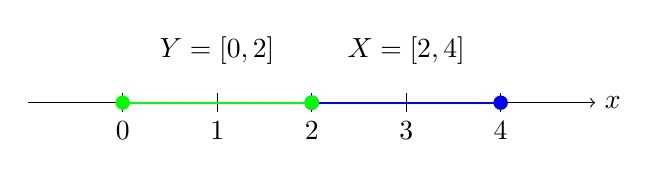
\begin{tikzpicture}[scale=1.2]
            % Number line
            \draw[->] (-1,0) -- (5,0) node[right] {$x$};
            
            % Labels
            \foreach \x in {0,1,2,3,4} {
                \draw (\x,0.1) -- (\x,-0.1) node[below] {\x};
            }
            
            % X Interval [2, 4] - Blue
            \draw[thick, blue] (2,0) -- (4,0);
            \filldraw[blue] (2,0) circle (2pt);
            \filldraw[blue] (4,0) circle (2pt);
            \node[above] at (3,0.3) {$X = [2, 4]$};
            
            % Y Interval [0, 2] - Green
            \draw[thick, green] (0,0) -- (2,0);
            \filldraw[green] (0,0) circle (2pt);
            \filldraw[green] (2,0) circle (2pt);
            \node[above] at (1,0.3) {$Y = [0, 2]$};
        \end{tikzpicture}
    \end{center}
    
    \begin{center}
        % Second number line showing the union interval
        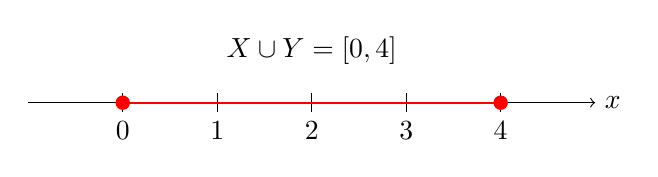
\begin{tikzpicture}[scale=1.2]
            % Number line
            \draw[->] (-1,0) -- (5,0) node[right] {$x$};
            
            % Labels
            \foreach \x in {0,1,2,3,4} {
                \draw (\x,0.1) -- (\x,-0.1) node[below] {\x};
            }
            
            % Union Interval [0, 4] - Red
            \draw[thick, red] (0,0) -- (4,0);
            \filldraw[red] (0,0) circle (2pt);
            \filldraw[red] (4,0) circle (2pt);
            \node[above] at (2,0.3) {$X \cup Y = [0, 4]$};
        \end{tikzpicture}
    \end{center}
\end{example}    

\begin{example}
    Now, consider the intervals \( A = \left[1, 3\right] \) and \( B = \left[5, 7\right] \), which do not overlap. In set-builder notation, these intervals are represented as:  
    \[
    A = \{x \in \mathbb{R} \mid 1 \leq x \leq 3\}, \quad B = \{x \in \mathbb{R} \mid 5 \leq x \leq 7\}.
    \]
    
    The union \( A \cup B \) consists of all numbers that belong to either interval. Since the intervals do not overlap, the union keeps both ranges separate:  
    \[
    A \cup B = \{x \in \mathbb{R} \mid 1 \leq x \leq 3 \text{ or } 5 \leq x \leq 7\}.
    \]
    
    Thus, the union contains two separate intervals: \([1, 3]\) and \([5, 7]\).
    
    \begin{center}
        % First number line showing A and B intervals
        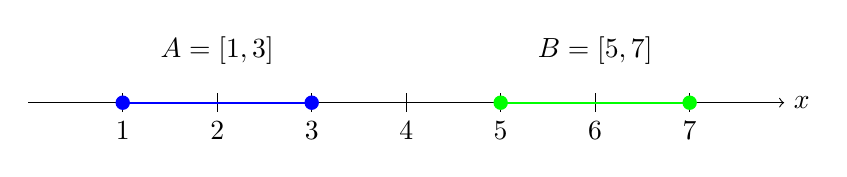
\begin{tikzpicture}[scale=1.2]
            % Number line
            \draw[->] (0,0) -- (8,0) node[right] {$x$};
            
            % Labels
            \foreach \x in {1,2,3,4,5,6,7} {
                \draw (\x,0.1) -- (\x,-0.1) node[below] {\x};
            }
            
            % A Interval [1, 3] - Blue
            \draw[thick, blue] (1,0) -- (3,0);
            \filldraw[blue] (1,0) circle (2pt);
            \filldraw[blue] (3,0) circle (2pt);
            \node[above] at (2,0.3) {$A = [1, 3]$};
            
            % B Interval [5, 7] - Green
            \draw[thick, green] (5,0) -- (7,0);
            \filldraw[green] (5,0) circle (2pt);
            \filldraw[green] (7,0) circle (2pt);
            \node[above] at (6,0.3) {$B = [5, 7]$};
        \end{tikzpicture}
    \end{center}
    
    \begin{center}
        % Second number line showing the union interval with a gap
        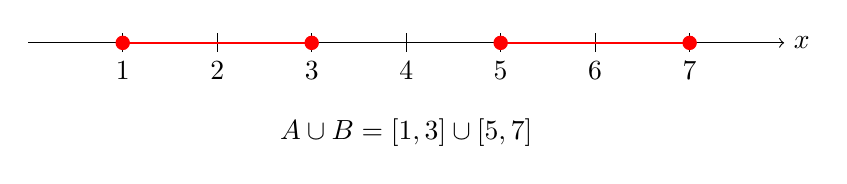
\begin{tikzpicture}[scale=1.2]
            % Number line
            \draw[->] (0,0) -- (8,0) node[right] {$x$};
            
            % Labels
            \foreach \x in {1,2,3,4,5,6,7} {
                \draw (\x,0.1) -- (\x,-0.1) node[below] {\x};
            }
            
            % Union Interval [1, 3] - Red
            \draw[thick, red] (1,0) -- (3,0);
            \filldraw[red] (1,0) circle (2pt);
            \filldraw[red] (3,0) circle (2pt);
            
            % Union Interval [5, 7] - Red
            \draw[thick, red] (5,0) -- (7,0);
            \filldraw[red] (5,0) circle (2pt);
            \filldraw[red] (7,0) circle (2pt);
            
            % Label for the union
            \node[above] at (4,-1.2) {$A \cup B = [1, 3] \cup [5, 7]$};
        \end{tikzpicture}
    \end{center}
\end{example}


\begin{definitionbox}{Intersection of Two Sets}  
    The \textbf{intersection of two sets} is the set containing all elements that are present in both sets. It is denoted by \( A \cap B \). In set-builder notation, the intersection can be written as:  
    \[
    A \cap B = \{x \mid x \in A \text{ and } x \in B\}.
    \]
    
    The intersection contains only the elements that both sets have in common. If two sets have no elements in common, their intersection is the empty set, denoted by \( \emptyset \). In this case, we say that the sets are \textit{disjoint} or \textit{non-intersecting}.
\end{definitionbox}    

\begin{example}
    Let \( A = \{1, 2, 3, 4\} \) and \( B = \{3, 4, 5, 6\} \). The intersection \( A \cap B \) consists of all elements that are present in both sets:  
    \[
    A \cap B = \{3, 4\}.
    \]
    
    \textbf{Explanation:} The numbers 3 and 4 are the only elements that both sets have in common.
\end{example}    

\begin{example}
    Consider the intervals \( A = \left[1, 5\right] \) and \( B = \left[3, 7\right] \). In set-builder notation:  
    \[
    A = \{x \in \mathbb{R} \mid 1 \leq x \leq 5\}, \quad B = \{x \in \mathbb{R} \mid 3 \leq x \leq 7\}.
    \]
    
    The intersection \( A \cap B \) consists of all numbers that belong to both intervals:  
    \[
    A \cap B = \{x \in \mathbb{R} \mid 3 \leq x \leq 5\}.
    \]
\end{example}

\begin{example}
    Consider some arbitrary set \(Z\) and the empty set \(\emptyset\). Then \(Z \cap \emptyset = \emptyset\), because there are no elements that are in both sets.
\end{example}

\begin{definitionbox}{Set Difference}  
    The \textbf{difference of two sets} \( A \setminus B \) is the set of all elements that belong to \( A \) but not to \( B \). In set-builder notation, it is written as:  
    \[
    A \setminus B = \{x \mid x \in A \text{ and } x \notin B\}.
    \]
    
    The set difference operation removes from \( A \) any elements that are also present in \( B \).
\end{definitionbox}

\begin{example}
    Consider the intervals \( A = \left[1, 5\right] \) and \( B = \left[3, 7\right] \). In set-builder notation:  
    \[
    A = \{x \in \mathbb{R} \mid 1 \leq x \leq 5\}, \quad B = \{x \in \mathbb{R} \mid 3 \leq x \leq 7\}.
    \]
    
    The difference \( A \setminus B \) consists of all numbers that belong to \( A \) but not to \( B \):  
    \[
    A \setminus B = \{x \in \mathbb{R} \mid 1 \leq x < 3\}.
    \]
\end{example}

\section{De Morgan's Laws}

When working with unions and intersections of sets, we often need to find the difference between a set and a combined set. In such cases, \textbf{De Morgan's Laws} help simplify expressions involving set differences.

\begin{theorembox}{De Morgan's Laws}
Let \( A \), \( B \), and \( C \) be any sets. Then the following statements hold:
    \begin{itemize}
    \item \( A \setminus (B \cup C) = (A \setminus B) \cap (A \setminus C) \),
    \item \( A \setminus (B \cap C) = (A \setminus B) \cup (A \setminus C) \).
    \end{itemize}
\end{theorembox}

\begin{proof}
    We will prove both statements using set difference and basic set properties.

    \begin{enumerate}
        \item \textbf{Proof of \( A \setminus (B \cup C) = (A \setminus B) \cap (A \setminus C) \):}
    
        Let \( x \in A \setminus (B \cup C) \). This means:
        \[
        x \in A \quad \text{and} \quad x \notin (B \cup C).
        \]
        The condition \( x \notin (B \cup C) \) implies that \( x \notin B \) and \( x \notin C \).
        
        Thus:
        \[
        x \in A \quad \text{and} \quad x \notin B \quad \text{and} \quad x \notin C.
        \]
        
        By the definition of set difference, this means:
        \[
        x \in (A \setminus B) \quad \text{and} \quad x \in (A \setminus C).
        \]
        
        Therefore:
        \[
        x \in (A \setminus B) \cap (A \setminus C).
        \]
        
        Now, let \( x \in (A \setminus B) \cap (A \setminus C) \). This means:
        \[
        x \in (A \setminus B) \quad \text{and} \quad x \in (A \setminus C).
        \]
        
        So:
        \[
        x \in A, \quad x \notin B, \quad \text{and} \quad x \notin C.
        \]
        
        Therefore:
        \[
        x \notin (B \cup C),
        \]
        which implies:
        \[
        x \in A \setminus (B \cup C).
        \]
        
        Thus, we have shown that:
        \[
        A \setminus (B \cup C) = (A \setminus B) \cap (A \setminus C).
        \]

        \item \textbf{Proof of \( A \setminus (B \cap C) = (A \setminus B) \cup (A \setminus C) \):}
    
        Let \( x \in A \setminus (B \cap C) \). This means:
        \[
        x \in A \quad \text{and} \quad x \notin (B \cap C).
        \]
        The condition \( x \notin (B \cap C) \) implies that either \( x \notin B \) or \( x \notin C \).
        
        Thus:
        \[
        x \in A \quad \text{and} \quad (x \notin B \quad \text{or} \quad x \notin C).
        \]
        
        This means that either:
        \[
        x \in (A \setminus B) \quad \text{or} \quad x \in (A \setminus C).
        \]
        
        Therefore:
        \[
        x \in (A \setminus B) \cup (A \setminus C).
        \]
        
        Now, let \( x \in (A \setminus B) \cup (A \setminus C) \). This means that either:
        \[
        x \in (A \setminus B) \quad \text{or} \quad x \in (A \setminus C).
        \]
        
        In both cases, we have:
        \[
        x \in A \quad \text{and} \quad x \notin (B \cap C).
        \]
        
        Therefore:
        \[
        x \in A \setminus (B \cap C).
        \]
        
        Thus, we have shown that:
        \[
        A \setminus (B \cap C) = (A \setminus B) \cup (A \setminus C).
        \]
    \end{enumerate}
    
    This completes the proof of both statements.
\end{proof}    

\section{Algebraic Properties}

There are various \textit{algebraic properties} that mathematical objects and operations can have. To better understand how these operations behave, we need some terminology to describe their behavior. 

For example, if an operation \( * \) is defined on some objects \( X \) and \( Y \), and swapping the order of the objects doesn’t change the result — that is, if \( X * Y = Y * X \) — we say the operation is \textit{commutative}.

In this section, we’ll go over some fundamental algebraic properties that operations on sets, numbers, or other mathematical structures can satisfy.

\begin{definitionbox}{Commutativity}
    An operation is called \textbf{commutative} if changing the order of the objects does not change the result. Formally, an operation \( * \) is commutative if:  
    \[
    X * Y = Y * X
    \]
    for any objects \( X \) and \( Y \) in the set where the operation is defined.
\end{definitionbox}

\begin{example}
    The operations of \textbf{addition} and \textbf{multiplication} of two numbers are commutative. That is, changing the order of the numbers does not change the result.
    
    For example:
    \[
    2 + 4 = 4 + 2, \quad \text{and} \quad 2 \cdot 4 = 4 \cdot 2.
    \]
    
    More generally, for any two numbers \( a \) and \( b \):
    \[
    a + b = b + a, \quad \text{and} \quad a \cdot b = b \cdot a.
    \]
    
    However, subtraction and division are \textbf{not} commutative. For instance:
    \[
    5 - 3 \neq 3 - 5, \quad \text{and} \quad 6 \div 2 \neq 2 \div 6.
    \]

    \textit{Remark: The set of real numbers, along with addition and multiplication, forms an algebraic structure called a "Field." We will explore fields and their properties in more detail later.}
\end{example}

\begin{example}
    The operations of \textbf{union} and \textbf{intersection} of two sets are \textbf{commutative}. This means that the order in which the sets are combined does not affect the result.
    
    For example:
    \[
    \{1, 2, 3\} \cup \{3, 4, 5\} = \{3, 4, 5\} \cup \{1, 2, 3\},
    \]
    and:
    \[
    \{1, 2, 3\} \cap \{3, 4, 5\} = \{3, 4, 5\} \cap \{1, 2, 3\}.
    \]
    
    More generally, for any two sets \( A \) and \( B \):
    \[
    A \cup B = B \cup A, \quad \text{and} \quad A \cap B = B \cap A.
    \]
    
    However, the \textbf{difference} operation is \textbf{not} commutative. For instance:
    \[
    \{1, 2, 3\} \setminus \{3, 4, 5\} \neq \{3, 4, 5\} \setminus \{1, 2, 3\}.
    \]
\end{example}

\begin{definitionbox}{Associativity}
    An operation is called \textbf{associative} if putting objects inside brackets (or parentheses) in different ways does not change the result. In other words, the way we group the objects does not affect the outcome of the operation.
    
    \textbf{Formally:}  
    An operation \( * \) is associative if, for any objects \( X \), \( Y \), and \( Z \) in the set where the operation is defined:
    \[
    (X * Y) * Z = X * (Y * Z).
    \]
\end{definitionbox}

\begin{example}
    The operations of \textbf{addition} and \textbf{multiplication} of numbers are associative. For instance:
    \[
    (2 + 3) + 4 = 2 + (3 + 4),
    \]
    and:
    \[
    (1 \times 2) \times 3 = 1 \times (2 \times 3).
    \]
    
    However, \textbf{subtraction} and \textbf{division} are \textbf{not} associative. For example:
    \[
    (5 - 3) - 1 \neq 5 - (3 - 1),
    \]
    and:
    \[
    (8 \div 4) \div 2 \neq 8 \div (4 \div 2).
    \]
\end{example}

\begin{example}
    In set operations, both \textbf{union} and \textbf{intersection} are associative.
    
    For any sets \( A \), \( B \), and \( C \):
    \[
    (A \cup B) \cup C = A \cup (B \cup C),
    \]
    and:
    \[
    (A \cap B) \cap C = A \cap (B \cap C).
    \]
    
    This means we can perform unions or intersections in any order without affecting the result.
\end{example}    

\begin{definitionbox}{Identity Element}
    An operation \( * \) is said to have an \textbf{identity element} if there exists an object \( e \) such that, for any object \( X \) in the set where the operation is defined:
    \[
    X * e = X \quad \text{and} \quad e * X = X.
    \]
    
    The identity element leaves any object "unchanged" under the operation.
\end{definitionbox}

\begin{example}
    In the case of numbers, the number \( 0 \) is called the \textit{additive identity} because adding it to any number doesn’t change the number:
    \[
    a + 0 = 0 + a = a.
    \]
    
    Similarly, the number \( 1 \) is called the \textit{multiplicative identity} because multiplying any number by \( 1 \) leaves it unchanged:
    \[
    a \cdot 1 = 1 \cdot a = a.
    \]
    
    For example:
    \[
    2 + 0 = 2, \quad \text{and} \quad 2 \cdot 1 = 2.
    \]
\end{example}            

\begin{example}
    In the case of set operations, the \(\emptyset\) (empty set) is the \textit{identity element for union}. For any set \( A \), taking the union with the empty set doesn’t change the set:
    \[
    A \cup \emptyset = \emptyset \cup A = A.
    \]
    
    Similarly, the \textit{universal set} \( U \) (a set that contains all elements in the context) is the \textit{identity element for intersection}, because intersecting any set with \( U \) leaves the set unchanged:
    \[
    A \cap U = U \cap A = A.
    \]
    
    For example, if \( A = \{1, 2, 3\} \) and \( U = \{1, 2, 3, 4, 5\} \), then:
    \[
    A \cup \emptyset = \{1, 2, 3\}, \quad \text{and} \quad A \cap U = \{1, 2, 3\}.
    \]
\end{example}        

\begin{definitionbox}{Inverse Element}
    An operation \( * \) is said to have an \textbf{inverse element} if, for any object \( X \) in the set where the operation is defined, there exists another object \( Y \) such that:
    \[
    X * Y = e \quad \text{and} \quad Y * X = e,
    \]
    where \( e \) is the identity element for that operation.
    
    The inverse element "undoes" the effect of the operation and returns the identity element.
\end{definitionbox}

\begin{example}
    The \textit{additive inverse} of the number \( 2 \) is \( -2 \), because adding them together gives the additive identity:
    \[
    2 + (-2) = 0,
    \]
    where \( 0 \) is the additive identity.
    
    Similarly, the \textit{multiplicative inverse} of the number \( 2 \) is \( 2^{-1} \) or \( \frac{1}{2} \), because multiplying them together gives the multiplicative identity:
    \[
    2 \cdot \frac{1}{2} = 1,
    \]
    where \( 1 \) is the multiplicative identity.
\end{example}    

\begin{definitionbox}{Distributivity}
    An operation \( * \) is said to be \textbf{distributive} over another operation \( \oplus \) if, for any objects \( X \), \( Y \), and \( Z \) in the set where the operations are defined:
    \[
    X * (Y \oplus Z) = (X * Y) \oplus (X * Z).
    \]
    
    This property means that applying the operation \( * \) to a combined object is the same as applying it separately to each part and then combining the results using \( \oplus \).
\end{definitionbox}

\begin{example}
    In the case of numbers, multiplication is \textit{distributive} over addition. This means multiplying a number by the sum of two numbers is the same as multiplying the number by each of them separately and then adding the results.
    
    For example:
    \[
    2 \cdot (3 + 4) = (2 \cdot 3) + (2 \cdot 4).
    \]
    
    Both sides simplify to:
    \[
    2 \cdot 7 = 6 + 8 = 14.
    \]
    
    More generally, for any numbers \( a \), \( b \), and \( c \):
    \[
    a \cdot (b + c) = (a \cdot b) + (a \cdot c).
    \]
\end{example}

\begin{example}
    In the case of set operations, the \textit{intersection} operation is \textit{distributive} over the \textit{union} operation. This means that intersecting a set with the union of two sets is the same as intersecting it with each set separately and then taking the union of the results.
    
    For example, for any sets \( A \), \( B \), and \( C \):
    \[
    A \cap (B \cup C) = (A \cap B) \cup (A \cap C).
    \]
    
    If:
    \[
    A = \{1, 2, 3\}, \quad B = \{2, 3, 4\}, \quad C = \{3, 4, 5\},
    \]
    then:
    \[
    A \cap (B \cup C) = \{2, 3\},
    \]
    and:
    \[
    (A \cap B) \cup (A \cap C) = \{2, 3\}.
    \]
    
    Both sides give the same result.
\end{example}